\documentclass[12pt]{article}

% Margins
\usepackage[letterpaper, top=1in, bottom=1in, left=.5in, right=.5in]{geometry}

% For prettier tables
\usepackage{array}

\usepackage{graphicx}

\usepackage{caption}

% For code
\usepackage{courier}
\usepackage{listings}
\lstset{ mathescape }
\lstset{basicstyle=\ttfamily\footnotesize,breaklines=true}

\usepackage{hyperref}

% Change Font
\usepackage[sfdefault]{roboto}  %% Option 'sfdefault' only if the base font of the document is to be sans serif
\usepackage[T1]{fontenc}

% For double spacing
\usepackage{setspace}

\usepackage[english]{babel}
\usepackage[utf8]{inputenc}
\usepackage{fancyhdr}

\pagenumbering{arabic}

\pagestyle{fancy}
\rhead{Jimmy Hickey}

\lhead{Intial Proposal}


%opening
\title{
Computer Corrected Color Blindness: Extended Proposal
}
\author{Jimmy Hickey}



\begin{document}
\maketitle
\doublespacing

\begin{abstract}
Many people suffer from color deficient vision; though they learn to cope, they still have many issues distinguishing between colors. In this paper, I propose a combination of computer vision and machine learning algorithms that can help eliminate some of the problems faced by color blind individuals. Through the methods such as edge detection and color recognition, this system will transform a given image into a more color blind friendly version.
\end{abstract}

\section{Introduction}

Color blindness is a deficiency in a person's color vision. A color blind person will often confuse different colors that a person with normal vision would not have trouble distinguishing. The most common type of color blindness is red-green, followed by blue-yellow, and the rare full lack of color vision. Red-green color blindness effects "as many as 8 percent of men and 0.5 percent of women with Northern European ancestry." (National Eye Institute) The effects of color blindness range from minor disruptions such as choosing a mismatched outfit to more major difficulties such as discerning between the colors of traffic lights.
There is no cure for color blindness, however there exist some methods to alleviate symptoms. 

One popular solution to color blindness is specialized glasses. The company enchroma sells a variety of these glasses. Color vision starts in the cones of the eye, of which people have three varieties: green, red, and blue. These detect and distinguish between different wavelengths of light; however, in the eye of a color blind person, this discrimination is not always made properly. The enchroma glasses filter out the overlapping wavelengths, making distinctions (particularly between red and green) clearer. These glasses range from \$349 to \$429 without prescriptions and are not ``intended to help pass color blindness tests for occupational purposes." (enchroma) Additionally, they (enchroma brand) are not useful to people with blue-yellow color blindness. A more permanent solution is currently being tested as well.

There is experimental gene therapy that has produced promising results in animals. In one study squirrel monkeys, which are naturally red-green color blind, were made able to perceive differences in the two colors after treatment. These animals were monitored and ``retained their new tricolor sensory capacity for more than two years." (MIT Technology Review). Additionally, there have been no detected harmful side effects from the treatment; four more animals have been successfully treated since. These auspicious trials suggest that there may be a permanent fix to color blindness in the near future; however, gene therapy is often prohibitively expensive, costings hundreds of thousands of dollars per patient. A short-term, cheap solution to some of the issues faced by the color blind is needed. 

The burgeoning field of computer vision lends itself perfectly to this problem. Much work has been done in the area of feature recognition. Projects like Google's deep dream and work in robotic vision are some of the wide applications of computer vision. Computers' abilities to analyze images is greatly enhancing. These methods can be used as the small, cheap fix to some color blind issues. A first step would be to examine images.

Instead of recognizing complex features, a machine needs only to examine the colors in an image. With appropriate knowledge of the problem domain, it should be able to diagnose whether there is areas of the image that may cause issues for the color blind. For example, given a set of color blind tests, it would be able to tell which slides a color blind person would have trouble with. This process can then be incrementally furthered.

\begin{enumerate}
	\item The system can mark all problem areas.
	\item The system can fix the problem areas without losing too much of the context of the image.
	\item The system can perform the preceding actions on a video.
	\item The system can perform the preceding actions on a live video feed.
\end{enumerate}

For the scope of this project, the first and second object will be addressed.

Unlike the glasses, the machine is not dealing with the light itself, but how it is displayed. Thus, this could be easily expanded to support all of the common types of color blindness. 


\section{Hypothesis}
A system can be trained to identify and resolve areas of potential color blind confusion in images.


\section{Methods}

\subsection{Data Creation}
\subsubsection{Image Creation}
Initially, it was planned to use standard Ishihara Color Test plates, such as those used by eye doctors, as the data for this experiment. See figure \ref{fig:ishi} for an example.

\begin{figure}[h]
	\centering
	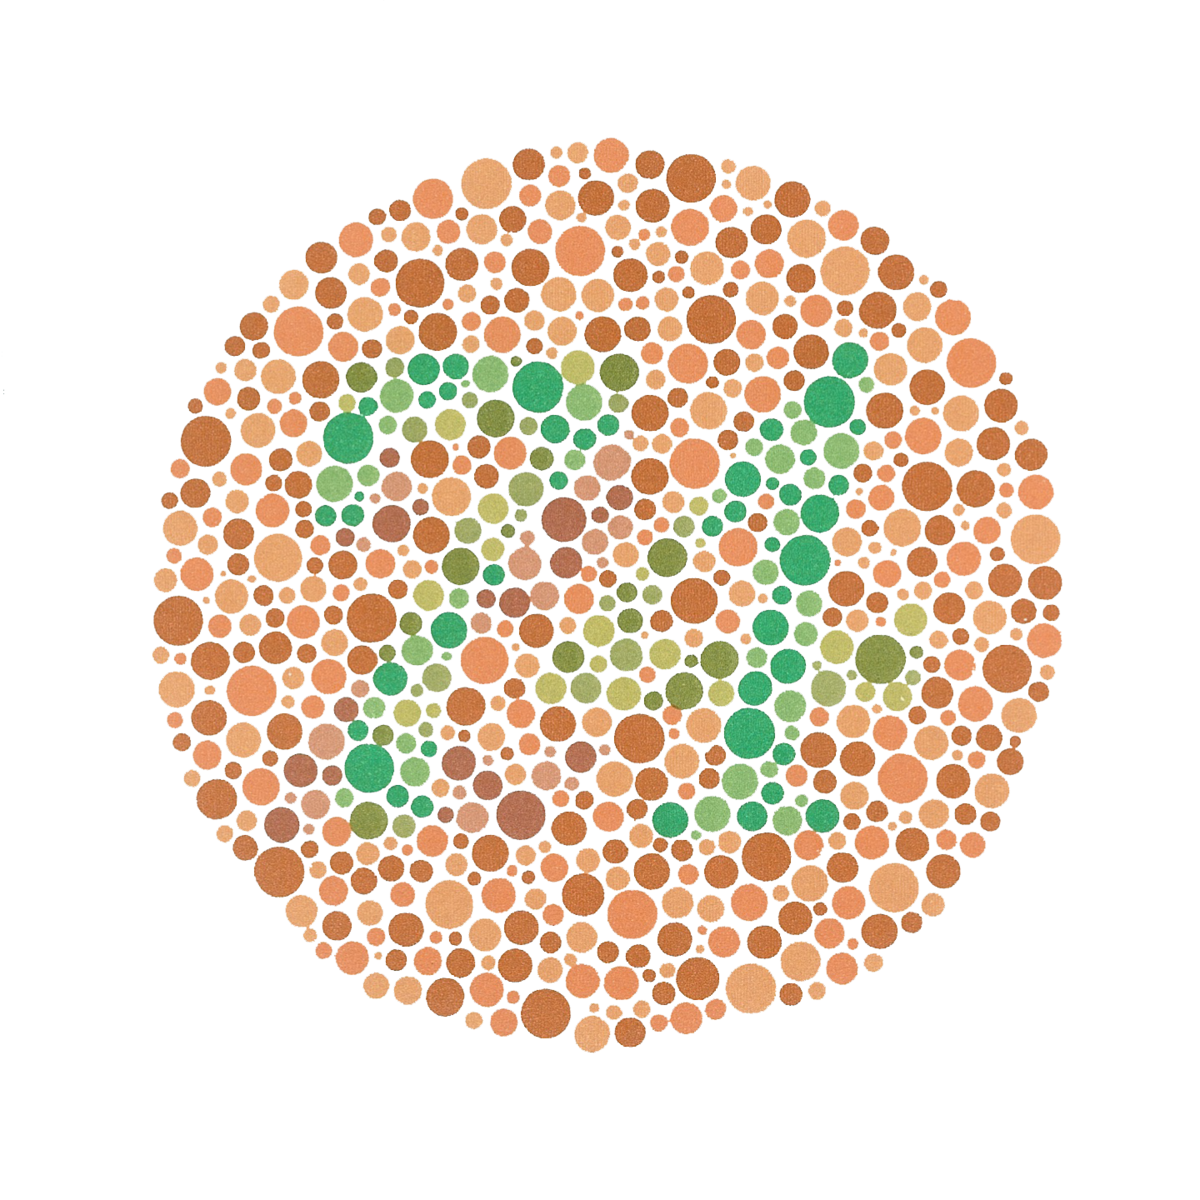
\includegraphics[width=0.25\textwidth]{img/Ishihara}
	\caption{A red-green Ishihara color blind plate.}
	\captionsetup{font={footnotesize,bf,it}}
	\caption*{\href{https://en.wikipedia.org/wiki/Ishihara\_test}{https://en.wikipedia.org/wiki/Ishihara\_test}}
	\label{fig:ishi}
\end{figure}

However, this afforded little control of the data. The learning process would rely on only the Ishihara samples publicly available online. 

Instead of this, new data was generated for the sake of this experiment. This allows for a wider range of data to be created and manipulated to help the system learn more color combinations. The data created using Adobe Illustrator. A background was chosen and then a foreground image was drawn. The colors of the background and foreground were tweaked until a red-green color blind person started having trouble distinguishing between the two. Figure \ref{fig:data1} shows pink sailboat on a gray background.

\begin{figure}[h]
	\centering
	
\includegraphics[width=0.25\textwidth]{img/data2.png}
	\caption{A sample data point.}
	\label{fig:data1}
\end{figure}

For a color blind person (particularly red-green color blind), it may be very difficult to discriminate between the background and foreground. This process will be continued to create a plethora of color combinations such as blue-purple, brown-red, orange-yellow, red-green, etc. These color combinations will then be altered and repeated. For example, dark blue and dark purple will be used in one image a lighter tint of each color will be used in another.

Issues with the devised data creation system will be explored in the Future Improvements section.

\subsubsection{Image Translation}
The image data needs to be represented in a more quantitative format while still maintaining the information stored in the picture. Namely, the infomration to retain is the color and location of each pixel. Thus, the x and y position will be stored as well as the blue, green, and red values for each pixel. Table \ref{table:1} shows a few rows of the data table representing the sailboat image from figure \ref{fig:data1}. 

\begin{table}[h!]
	\centering
	\begin{tabular}{ c c c c c}
		x & y & B & G & R \\\hline 
		0 & 0 & 205 & 205 & 205 \\  
		0 & 0 & 205 & 205 & 205 \\
		0 & 0 & 205 & 205 & 205 \\    
		&  & \vdots &  &  \\ 
		57 & 116 & 217 & 184 &233\\
		&  & \vdots &  &  \\ 
		0 & 0 & 205 & 205 & 205 \\		
	\end{tabular}
	\caption{Image representation of sail boat picture}
	\label{table:1}
\end{table}

\subsection{Color Detection}
Unsupervised learning algorithms including pattern recognition will be used to solve this problem. Differences in color could be detected in each image. A neural network will be used to find relationships between these problem colors.
Since multiple images will be created for each color combination, local maxima will, hopefully, be avoided. 

Here is a a brief summary of the anticipated process:
\begin{enumerate}
\item A data point is given to the system.
\item The system examines the hexademical color values of the pixels in the data point, storing the differences and relationships between them.
\item Steps 1 \& 2 are repeated for all data points.
\item With the full data set explored, the system will take the hexademical color values that it has found and try to use them to find patterns.
\end{enumerate}

It is expected that the system will identify issues with the red and green more so than the blue since it will be given data for a red-green color blind person.

\subsection{Color Correction}

One simple correction method that could be employed is through the use of edge detection. Once the system is properly trained to determine problem areas in images, an edge could be detected. Tracing this area with a thin black line would offer a visible separation between the two competing colors, while trying not to lose the information stored in the image.

Another possible correction procedure is to change the colors of the image itself. For example. in the sailboat data point in figure \ref{fig:data1}, the pink or the gray could be darkened. This method would leave the picture more intact as it wouldn't draw black lines everyone, which could make the image more cumbersome to look at. However, this color changing would have to be very precise as to not completely alter the image. Changing the boat to black would assuredly make it more visible, but the image is no longer of a pink boat and a gray background. Subtly changing the color values would ensure that the image is still in tact while being more accessible. With improvements to the system such as user testing this mechanism could be fine tuned to translate an image into a user and color blind friendly picture.
\section{Future Improvements}
The scope of this project has greatly limited its potential, however with some additions and changes it can be vastly improved.

\subsection{Better Data}
The data is currently created by one person that is red-green color blind. This is a humble start, everyone's color blindness is a little different. Thus, creating data that caters to only one person may leave out issues experienced by many other people with red-green and blue-yellow color deficiencies.

To solve this problem, the National Eye Institute or even an eye doctor could be inquired about the data. They could judge the data set created to see if there are any glaring cases missing from examination. Alternatively, they could provide the data themselves. These expert analysis of the problem would make the system more reliable.

\subsection{Including Users in the Development}
Any good software is going to include some sort of user testing. In this case, the users could help refine both the data and the correction functionality. Similar to an expert's opinion, getting feedback from many users will help create reliable data. This will ensure that no color combinations go un-learned by the system. 

After the system has learned with a more inclusive data set, the users could also help judge the color correction. They could be given before and after pictures; offering their input as to whether the system actually accomplished its goal of helping them distinguish the colors in the image. Additionally, a non-color blind group of people could be brought in, again given the before and after pictures. These participants would be able to determine how drastic a change the system made to the image. Combining feedback from these two groups of people would help reach an equilibrium between making an image more accessible while not altering its meaning.


\section{References}
\singlespacing
\textbf{BIBTEX TO COME!}
\begin{enumerate}
	\item 
		\href{https://nei.nih.gov/health/color_blindness/facts_about}{National Eye Institute}

	\item
		\href{https://www.technologyreview.com/s/601782/how-enchromas-glasses-correct-color-blindness/}{MIT Technology Review of Enchroma glasses}
	
	\item
		\href{http://enchroma.com/contact-us/}{Enchroma website}
		
	\item
		\href{https://www.technologyreview.com/s/415339/color-blind-monkeys-get-full-color-vision/}{MIT Technology Review of Color Blind Monkey Gene Therapy}
		


\end{enumerate}

\end{document}
